\documentclass{cslthse-msc}
\usepackage[utf8]{inputenc}
\usepackage[english]{babel}
\usepackage{amsmath}
\usepackage{amsfonts}
\usepackage{amssymb}
\usepackage{amsthm}
%\usepackage{makeidx}
\usepackage{graphicx}
\usepackage[titletoc, header, page]{appendix}
\usepackage{todo}

\usepackage[hidelinks]{hyperref}

\author{
	Alexander Söderberg \\
	{\normalsize \href{mailto:email@alexandersoderberg.com}{\texttt{email@alexandersoderberg.com}}}
	\and
	Max Åberg \\
    {\normalsize \href{mailto:aaberg.max@gmail.com}{\texttt{aaberg.max@gmail.com}}}
}

\title{Optimizing business intelligence
extraction speed from an
ERP-system’s database}
\subtitle{Master Thesis}
\company{Perfect IT BeX AB}
\supervisors{Lennart Söderberg, \href{mailto:lennart@perfectit.se}{\texttt{lennart@perfectit.se}}}{Alma Orucevic Alagic, \href{mailto:alma@cs.lth.se}{\texttt{alma@cs.lth.se}}}
%\supervisor{John Deer, \href{mailto:jdeer@company.com}{\texttt{jdeer@company.com}}}
\examiner{Per Andersson, \href{mailto:per.andersson@cs.lth.se}{\texttt{per.andersson@cs.lth.se}}}

\date{\today}

\acknowledgements{
\todo{Skriv acknowledgements}
}

\theabstract{
\todo {Skriv abstract}

}

\keywords{MSc, MsSQL, ERP, Optimization}

%% Only used to display font sizes
\makeatletter
\newcommand\thefontsize[1]{{#1 \f@size pt\par}}
\makeatother
%%%%%%%%%%


\begin{document}
\makefrontmatter
\chapter[Introduction]{Introduction}
2014 was the year of the cloud. Software companies strived to make their services cloud based in order to meet the increasing demands from the market of availability and reliability. 
In today's businesses there's high demand for accurate and up-to-date business intelligence.

\chapter{Background}
\section{Background}

\section{Problem description}
\section{Thesis Goals}'


\section{Scope}
The time frame of a master thesis is limited and therefore work limitations have to exist. The system consists of several essential parts, all of which can be optimized in different extent. The focus of this thesis's is speed optimization of business intelligence reports and therefore the following limitations have been established:
\begin{itemize}
\item The optimization will not effect the systems front-end other than the speed of report generation.
\item The optimization will not effect the original structure of the systems database.
\item The optimization will not change the logic of the queries made by the back-end to the database.
\item The optimization should be versatile enough to handle future database expansions and higher performance of the system. However, in the scope of this master thesis only estimations based on the current system can be done.
\end{itemize}

\section{Related Work}
\section{Contributions}

\chapter{Research Questions \& Methodology}
\section{Research Questions}
\section{Methodology}
\section{Work}

\chapter{Approach}
\section{Technical Description}
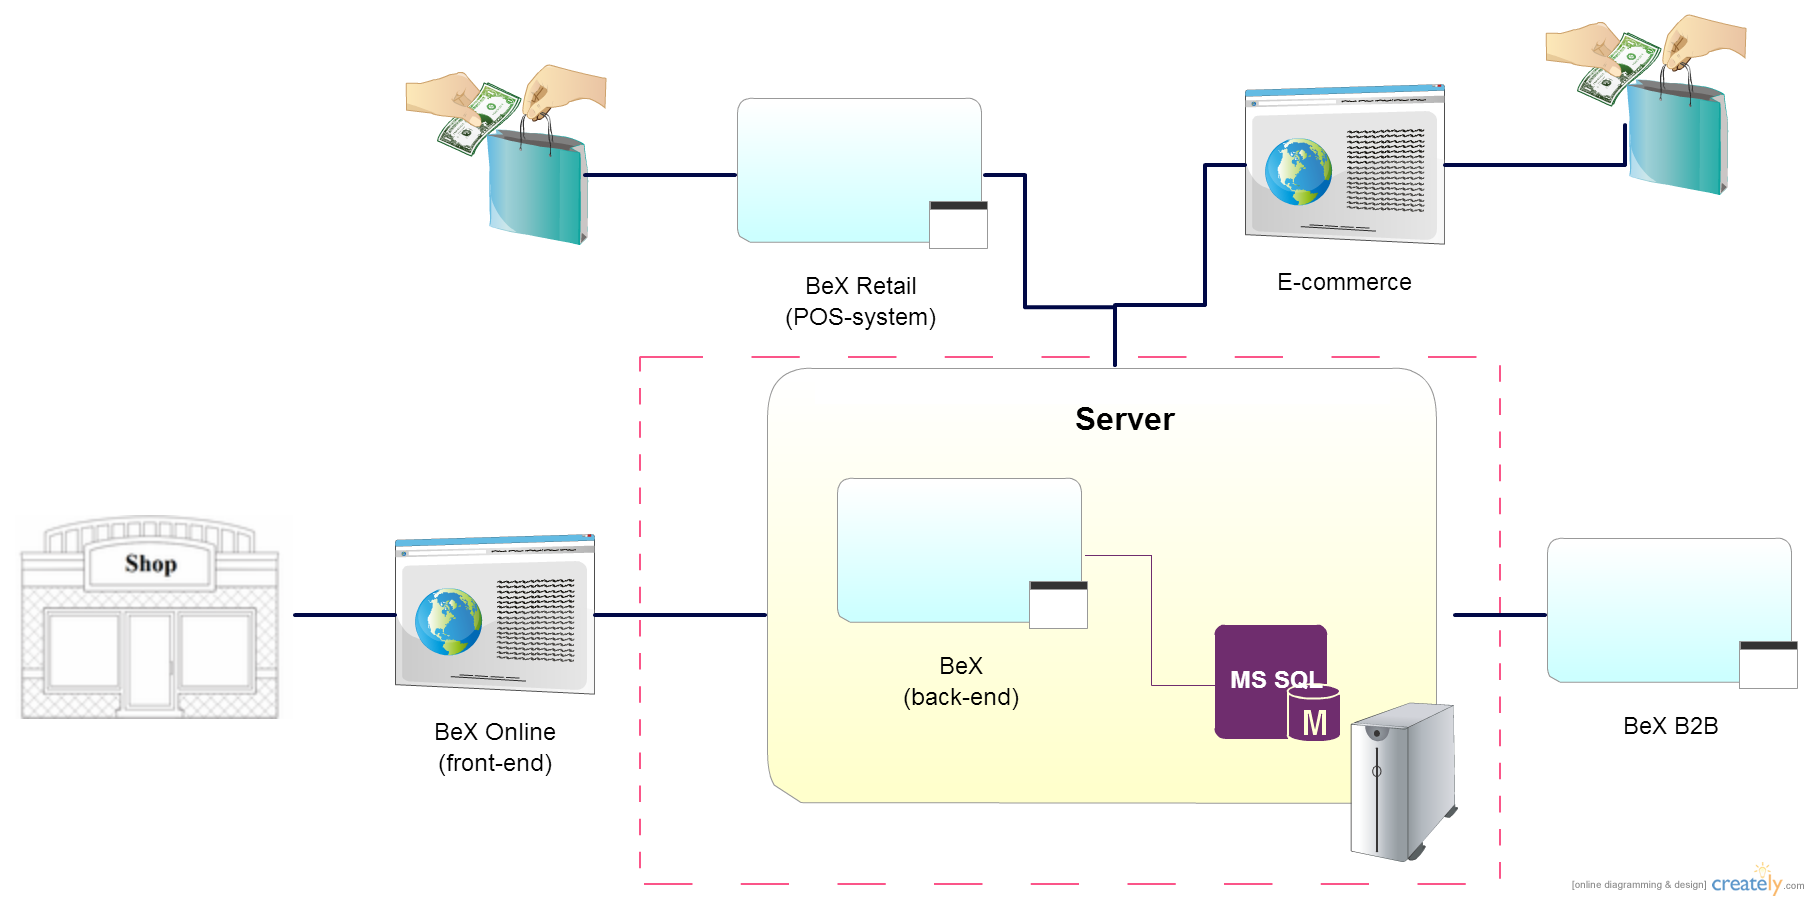
\includegraphics[scale=.2]{Systemdesc.png}
\section{Database}
\href{https://drive.google.com/file/d/0B1IYTmE2hnD-eGQ0N2tvYXZNNVE/view?usp=sharing}{Database schema link}

\section{Theory}
In order to understand why a database might not perform optimally, the following theory was used.
\subsection{Index Fragmentation}
Index fragmentation is one of the most common problems in a relational database. Two kinds of fragmentation can occur, internal index fragmentation and external index fragmentation. The easiest way to explain index fragmentation is by imagining the SQL database as a phone book. At the very end of the book you have a few pages containing a table with indexes of all the entries sorted by last name. This is fine in a static environment such as a phonebook but what happens in a dynamic environment?
Since people can be added to the phonebook there must be space available after each column in the index, as well as in the pages in the phonebook. This is called the fill factor. A page can still run out of space and when this happens SQL Server has to add a new page, but it it can't add it at the correct place beacause the book is already bound. So, it adds a blank page at the very end.
\section{Analysis}


\chapter{Proposed Solution}
\section{Solution Introduction}
\section{Integration}

\chapter{Software Development \& Testing}

\chapter{Discussion}

\chapter{Conclusions}

\bibliographystyle{plain}
\bibliography{MyMSc}
\end{document}
